\documentclass{article}
\usepackage[utf8x]{inputenc}
\usepackage[T1]{fontenc}
\usepackage[francais]{babel}

\usepackage{amsmath}
\usepackage{amsfonts}
\usepackage{amssymb}


\usepackage{mathpazo}

\usepackage{graphicx}
\usepackage{url}
\usepackage{listings}
%Le package listings n'est utilisé que pour le langage C
\lstset{ %
language=C,        % choix du langage
basicstyle=\footnotesize,       % taille de la police du code
numbers=left,                   % placer les numéros de lignes à droite (right) ou à gauche (left)
numberstyle=\normalsize,        % taille de la police des numéros
numbersep=7pt,                  % distance entre le code et sa numérotation
%backgroundcolor=\color{white},  % Couleur du fond. Possibilité d’utilisation du package color
}


\author{Pierre \bsc{Donat-Bouillud}}
\title{\emph{BlenderOS}}
\begin{document}
\maketitle

\section*{Introduction}
\emph{BlenderOS} est un système d'exploitation conçu spécialement pour exécuter Blender, logiciel open-source de création, édition d'images de synthèse, dans des conditions optimales, d'abord son moteur de rendu, et plus généralement les logiciels mettant en jeu des calculs portant sur le graphisme. Il est ainsi conçu pour une rapide vitesse d'exécution, et pour un support natif du calcul distribué. \emph{BlenderOS} peut se voir ainsi ajouté des capacités de calcul ou de connectique à l'aide de système clients qui peuvent être installés sur d'autres systèmes d'exploitation, ou former avec plusieurs autres instances distantes une grappe formant une entité unique. Il est ainsi le terrain d'expérimentation des algorithmes les plus sophistiqués, et, on le souhaite, les plus performants.
  
  Il est destiné à fonctionner sur des architectures 32 ou 64 bits, d'abord sur processeur Intel. L'implémentation de l'utilisation des ressources de la carte graphique à des fins de calculs pas forcément graphiques est envisagée au niveau du noyau. le système de clients de calcul permettra aussi d'accéder à des périphériques distants, ce qui assurera une compatibilité importante avec le matériel, tandis que les pilotes des périphériques cruciaux seront réécris pour une meilleure interaction avec Blender.

  \emph{BlenderOS} est aussi destiné à être lancé d'un cédérom, ou mieux, d'une clé USB, même si une installation sur disque est parfaitement possible, et même conseillé dans le cas d'une utilisation prolongée.
  
  \emph{BlenderOS} est inspiré, au moins dans quelques mécanismes bas niveau comme le chargement du noyau, par le noyau Pépin, dont le site à l'adresse suivante \url{http://a.michelizza.free.fr/pmwiki.php?n=TutoOS.TutoOS} décrit les étapes menant à un système basique, mais fonctionnel.


\part{Description}

\section{Architecture globale}

  Pour de meilleurs performances, \emph{BlenderOS} utilise un noyau monolithique. \emph{BlenderOS} désignera dorénavant tout aussi bien le noyau que le système d'exploitation, sans autre précision que l'apport éclairant du contexte.

\section{Le chargement du noyau}
  Le noyau répond au standard \emph{multiboot}. Il peut donc être lancé grâce à tout chargeur répondant à ce type de standard. \emph{Grub} est le chargeur privilégié.
 
\subsection{Le standard \emph{multiboot} }
  Pour répondre à ce standard, le noyau doit être pourvu de deux caractéristiques :
  \begin{itemize}
  	\item être un fichier exécutable 32 ou 64 bits standard
  	\item l'image du noyau doit contenir un entête spécial, le \emph{multiboot} header.
  \end{itemize}
  \paragraph*{Le \emph{multiboot} header}
  \begin{verbatim}
  global _start, start
extern kmain
   
%define MULTIBOOT_HEADER_MAGIC  0x1BADB002
%define MULTIBOOT_HEADER_FLAGS  0x00000003
%define CHECKSUM -(MULTIBOOT_HEADER_MAGIC + MULTIBOOT_HEADER_FLAGS)


_start:
        jmp start

; The Multiboot header
align 4
multiboot_header:
dd MULTIBOOT_HEADER_MAGIC
dd MULTIBOOT_HEADER_FLAGS
dd CHECKSUM    
; ----- Multiboot Header Ends Here -----

start:
        push ebx
        call kmain

        cli ; stop interrupts
        hlt ; halt the CPU
  \end{verbatim}

  Le \emph{multiboot} header résultant doit être placé au début du noyau grâce à une option appropriée du linker.
  
 \emph{Grub} peut aussi fournir au noyau la quantité de mémoire utilisée.
 
 La commande \emph{mbchk} de vérifier le conformité du noyau avec le standard \emph{multiboot} :
 \begin{verbatim}
 \$ mbchk kernel
	kernel: The Multiboot header is found at the offset 4104.
	kernel: Page alignment is turned on.
	kernel: Memory information is turned on.
	kernel: Address fields is turned off.
	kernel: All checks passed.

 \end{verbatim}

\section{La gestion de la mémoire}

  La gestion de la mémoire est une fonction cruciale d'un système d'exploitation. Elle doit répondre à deux problématiques :
  \begin{description}
  \item[être performante :] l'allocation de mémoire est une opération fondamentale, effectuée très régulièrement par l'ensemble des programmes exécutés sur le système
  \item[éviter la fragmentation :] la fragmentation apparaît lorsque des blocs de mémoire sont libérés mais ne sont pas utilisés car trop petits pour les demandes actuelles. Il en résulte un progressif gaspillage d'espace, et une recherche plus lente d'espace libre.
  \end{description}
  Une autre problématique, mineure, est de faire en sorte que la gestion de la mémoire ne vampirise pas toute la mémoire disponible, que les structures de gestion soient raisonnablement négligeables face à l'ensemble de la mémoire. Une autre est de permettre un accés séquentiel rapide à la mémoire.

\subsection{\textsl{Pré-requis :} connaître la taille de la mémoire disponible}
  \emph{BlenderOS} répond au standard \emph{multiboot} : le \emph{bootloader} que celui-ci met à disposition peut passer au noyau la taille de la mémoire disponible, qu'il a lui-même obtenu du \emph{BIOS}. Ainsi, \emph{Grub} transmet au noyau via la structure 
\verb|struct mb_partial_info| des informations, en particulier sur la mémoire.
\begin{lstlisting}
struct mb_partial_info {
        unsigned long flags;
        unsigned long low_mem;
        unsigned long high_mem;
        unsigned long boot_device;
        unsigned long cmdline;
};
\end{lstlisting}
  La structure complète contient d'autres informations telles que la carte de description de la mémoire initialisée par le \emph{BIOS}.
  Ces informations peuvent alors être utilisées ainsi : 
\begin{lstlisting}
void kmain(struct mb_partial_info *mbi)
{
        printk("Grub example kernel is loaded...\n");
        printk("RAM detected : %uk (lower), %uk (upper)\n", mbi->low_mem, mbi->high_mem);
        printk("Done.\n");
}
\end{lstlisting}

\paragraph*{TODO : } préciser le système de gestion utilisée : les adresses mémoires concrètes...\\

\subsection{Gestion de la mémoire physique}
  La mémoire est découpée en page de taille \emph{PAGESIZE}. L'allocation d'une page consiste à la marquée comme utilisée \emph{1}, ou libre \emph{0}, d'une façon comme d'une autre. Parmi différentes structures de données, comme une pile, ou une liste chainée, \emph{BlenderOS} utilise un système hybride formé d'une bitmap et d'un tas, tas en ce qu'il est stocké linéairement et qu'il est ordonné selon des adresses implicites. Chacun des bits de la bitmap représente l'état d'une page, de façon contiguë.
Cependant, un tel système se heurte au temps de recherche d'une page libre. En effet, on parcoure séquentiellement la bitmap jusqu'à trouver une page libre ; aussi dans le pire des cas, le temps de recherche est de $O(p)$ où $p$ est le nombre de pages du système. 

  Pour remédier à cette lenteur, la bitmap est divisée en blocs de taille $a$, référencés à l'aide d'un tas (arborescence complète) de hauteur $h$ tel que chacun de ses nœuds indiquent si les nœuds enfants comportent des blocs utilisés. 
Les feuilles du tas sont des pointeurs vers les différents blocs de la bitmap ; elles correspondent aux différents niveaux du tas. On peut donc accéder à un bloc de bits dès la racine, pas forcément au niveau de la feuille.

Pour accélérer plus encore le processus, on effectue un parcours non plus bit à bit, mais mot par mot, où un mot correspond à la taille du plus grand registre du microprocesseur, 32 bits, ou 64 bits. Si ce mot, en 32 bits, vaut 0xFFFFFFFF, c'est que ces 32 bits correspondent à 32 pages utilisées. Dans le cas contraire, on parcoure ces 32 bits à la recherche des bits à 0.

  Par ailleurs, il est probable, au moins au début avant fragmentation, que la page suivant la page couramment allouée soit une page libre. On garde donc un pointeur sur la page couramment allouée, et on teste avant tout parcours dans le tas si cette page suivante est libre. Cela ne rajoute qu'une seule opération. Cette heuristique accélère en particulier l'allocation d'une série de pages lors de demandes groupées par un programme.
  
  De même, chaque premier bit libre de chaque bloc est indiqué par un pointeur, à NULL s'il  n'y en a pas, mis à jour à chaque opération d'allocation ou suite groupée d'allocations.\\

  Ainsi, si dans le pire des cas, une allocation s'effectue en un temps $O(\ln p)$, dans le meilleur des cas, elle s'effectue en $O(1)$.
\begin{figure}[h]
\begin{center}
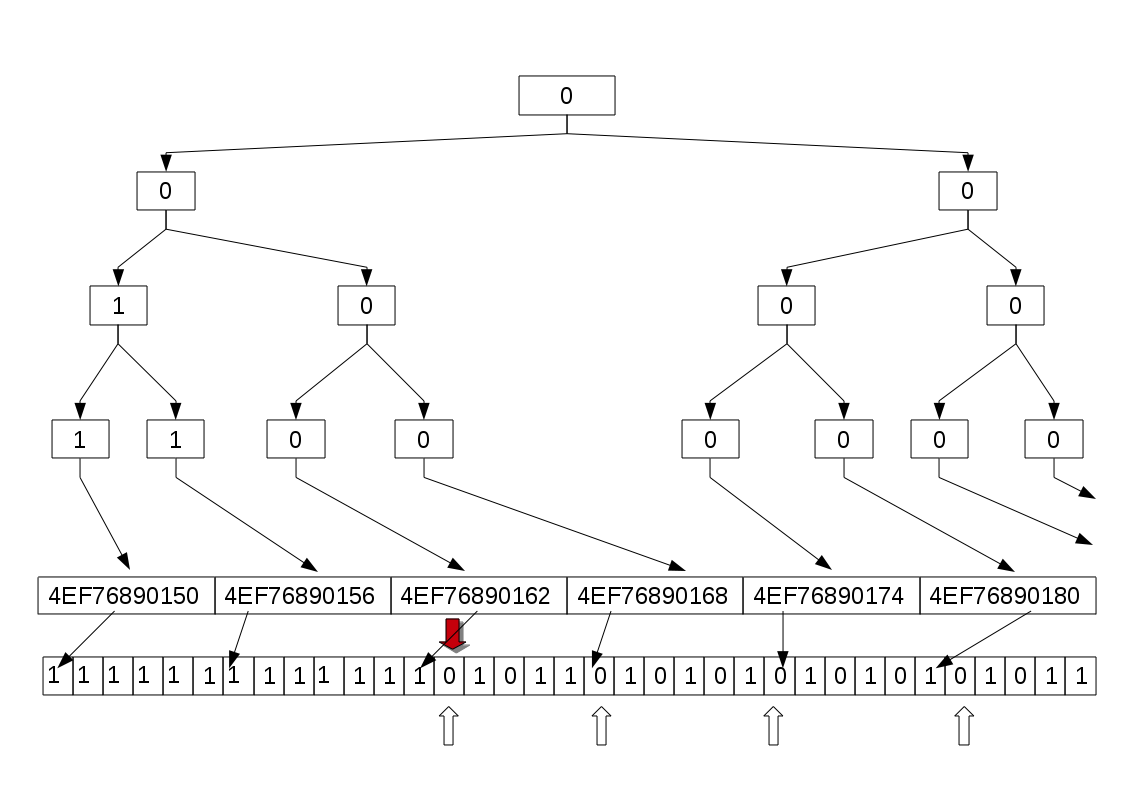
\includegraphics[scale=0.45]{AllocationPhysique-structure.png}
\end{center}
\caption{La structure du gestionnaire de mémoire physique}
\label{La structure du gestionnaire de mémoire physique}
\end{figure}

\paragraph*{Une structure à construire de façon optimale}
  On cherche à minimiser le temps de recherche d'une page libre. On appelle $h$ la hauteur de l'arborescence complète, $k$ le nombre d'enfants d'un nœuds, et $a$ la longueur d'un bloc, c'est-à-dire le nombre de pages qu'il peut décrire ; $n$ représente la taille de la mémoire physique, $t$, la taille d'une page.
  
  Calculons le nombre d'opérations que nécessite une recherche dans le pire des cas. L'arborescence $k$-aire de hauteur $h$ étant complète, elle compte $N_{k} = \frac{k^{h} -1 }{k-1}$ nœuds intérieurs et  $N_{h}$ feuilles, soit autant de blocs, où :
\begin{equation}
N_{h} = k^{h}
\end{equation}
Le nombre de pages $p$ total est :
\begin{equation}
p=\frac{n}{t}
\end{equation}
D'autre part, on peut exprimer ainsi le nombre total de pages :
\begin{equation}
p = N_{h} \times a = k^{h} \times a
\end{equation}
On en déduit l'égalité suivante :
\begin{equation}
a \times k^{h} = \frac{n}{t} \Leftrightarrow a = \frac{n}{t \times k^{h}}
\end{equation}
Le pire des cas n'advient pas lorsque la page suivant la page précédemment allouée est libre. 
On parcoure alors tous les enfants d'un nœud jusqu'à arriver à chaque fois au dernier enfant, puis arrivé au bloc, on le parcoure jusqu'à la fin.
\paragraph*{TODO :} revoir l'étude avec le pointeur de premier bit libre par bloc.  -> Abandonner ces pointeurs s'il n'y a que peu de blocs comme pour k=2.\\

La fonction qui modélise le nombre d'opérations dans le pire des cas est alors, en comptant la racine :
\begin{equation}
\Theta \left(h, k\right) = k \times h + a - 1= k \times h + \frac{n}{t \times k^{h}} + 1
\end{equation}
de dérivée partielle par rapport à $h$ : \[ \frac{\partial\Theta}{\partial h} = k - \frac{n \times \ln k \times k^{-h}}{t} \]
$\Theta$ atteint alors un minimum en :
\begin{equation}
h = \ln_{k} \frac{n \times \ln k}{t \times k} 
\end{equation}
Optimisons désormais : 
\[  \Xi \left(k\right) = \Theta \left( \ln_{k} \frac{n \times \ln k}{t \times k} , k \right) = \frac{k}{\ln k} \times \left( \ln \frac{n \times \ln k}{t \times k} + 1 \right) \]
La dérivée de $\Xi$ vaut :
\begin{equation}
\Xi'\left(k\right) =\frac{\ln k -1}{\ln^{2} k} \times \ln \frac{n \times \ln k}{t \times k}
\end{equation}
Elle s'annule en $ k = e \simeq 2.71$, le degré de l'arborescence étant une valeur entière, on peut choisir ou un arbre binaire, ou un arbre ternaire. L'arbre ternaire aura le degré le plus proche, le binaire, les opérations de navigation dans l'arbre les plus rapides, car obtenues par de simples décalages de bits et de $et$ binaires. $\Xi$ s'annule aussi  lorsque $ g : k \mapsto \frac{\ln k}{k} $ atteint  $ \frac{t}{n} $. Or $g$ a pour maximum
 $\frac{1}{e}$ en $e$. On doit donc avoir pour que ce membre s'annule : 
\begin{equation}
\frac{t}{n} \leqslant  \frac{1}{e}
\end{equation}
c'est-à-dire que :
\begin{equation}
\frac{t}{n} \lesssim 0.36 \ \%
\end{equation}
On appelle rapport critique de pagination $\mu_{P}$ ce rapport. Dans la majorité des cas, la taille d'une page est bien inférieure à la taille totale de la mémoire, et toujours en situation réelle, elle est inférieure à $\mu_{P}$. Par exemple, dans l'architecture
x86, en 32 bits, la taille d'une page est habituellement de 4 Ko, alors que la taille de la  mémoire peut atteindre les 4 Go, et dépasse toujours aujourd'hui pour les ordinateurs personnels les 512 Mo. 
\subparagraph*{Choix de $a$ et de $h$}
On utilise les équations déjà déterminées :
\begin{eqnarray}
h = \ln_{k} \frac{n \times \ln k}{t \times k} \\
a = \frac{k}{\ln k}
\end{eqnarray}
Par exemple, pour $k=2$, $n=4$ Go, et $t=4$ Ko, on a $h \simeq 18.47$, on choisit $h =18$, et $a \simeq 2.88$. On choisit $a=3$. En tout, on obtient $\Theta(18,3) = 39$ opérations dans le pire des cas.
Pour $k=3$, avec la même architecture de mémoire, $h=12$, et $a=3$, soit $\Theta(12, 3)=39$.
Il apparait donc plus tenant de choisir $k=2$.
%Choix de k entiérement à revoir (contre-exemple pour n=4 Go et t=4096 o): je trouve 10 comme valeur optimale de degré. On a alors h = 5.382 et a =4.3429. Cela vient probablement du fait que e est un maximum, tandis que k tel que ln k/k - t/n =0 correspondrait au minimum. A approfondir !
%Remarque fausse : oubli de multiplier par k la hauteur dans le calcul du nombre total d'opérations.
\paragraph*{TODO :} étude dans le cas moyen : considérer qu'une page est trouvée libre à peu près à la moitié d'un bloc. (en choisissant un politique first-ordered fit, c'est plus que probable : trouver une meilleure distribution -> exponentielle, de Poisson ??). Implémenter les deux stratégies, comparer les temps d'exécutions sur un programme réel.\\

\paragraph*{Allouer le gestionnaire de mémoire physique}
  Le gestionnaire de mémoire physique ne peut s'allouer lui-même : on retombe dans l'éternel problème du premier à voir le jour entre l'œuf et la poule !
  Il est donc directement placé en mémoire, à un emplacement stable, juste derrière le noyau.
\begin{figure}[h]
\begin{center}
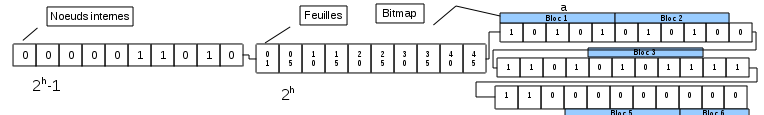
\includegraphics[scale=0.6]{AllocationPhysique-memoire.png}
\end{center}
\caption{L'emprise mémoire du gestionnaire de mémoire physique}
\label{L'emprise mémoire du gestionnaire de mémoire physique}
\end{figure}

\subsection{Gestion de la mémoire virtuelle}
\subsection{\textsl{Le cœur, crucial, de la gestion de l'allocation côté utilisateur :} \emph{malloc} et \emph{free}}
\subsection{\textsl{Gestion du manque de mémoire :} mémoire swap}


\part{Installation à partir des sources}

L'installation de \emph{BlenderOS} se fait à partir des sources, qu'il faudra compiler. Il faut ensuite créer une image où le noyau et grub sont correctement placés. On se propose de détailler les étapes menant à une installation propre, efficace, et durable de \emph{BlenderOS} à partir d'un système Linux. Un script permet aux néophytes d'accélérer le processus, au détriment des enseignements conséquents qui pourraient résulter d'une installation à la main.

\section{Compilation des sources}

  Positionner-vous dans le répertoire contenant les sources. Un simple \verb|make| permet de les compiler. Vous pouvez sélectionnez l'architecture à laquelle vous destinez votre futur système : 32 bits ou 64 bits.
  
\section{Installation de grub et du noyau de \emph{BlenderOS}}

\section{Installation des programmes complémentaires indispensables à l'administration et à l'exploitation du système}

\appendix

\section{Le standard \emph{multiboot}}
Cette annexe est une revue condensée et traduite en français de la spécification \emph{multiboot}.
 La spécification \emph{multiboot} veut unifier le chargement du noyau par une bootloader du point de vue du noyau lui-même : elle définit un header qui permet entre autres au noyau d'indiquer sa présence et l'adresse où il veut être chargé, un état dans lequel la machine doit se trouver lorsque le noyau est chargé, et enfin une structure passant de précieuses informations au noyau.
 
 \emph{BlenderOS} suit la spécification multiboot, et peut donc être lancé par \emph{Grub}.
 
\subsection{Le \emph{multiboot} header}
\subsection{Etat de la machine }
  Le registre EAX contient la valeur magique indiquant que le bootloader répond au standard \emph{multiboot}.
\subsection{La structure \emph{multiboot} information}
L'adresse de la structure d'informations sur le boot passée par le bootloader est stockée dans le registre EBX. Elle peut se trouver n'importe où dans la mémoire.
\begin{table}[h]
\begin{center}
\begin{tabular}{|c|c|c|}
\hline Offset & Contenu & Présence \\ 
\hline  O &  flags &  requis \\ 
\hline   4 & mem\_lower &  présent si flags[0] est activé \\ 
\hline  8 & mem\_upper &  présent si flags[0] est activé\\ 
\hline  12 & boot\_device & présent si flags[1] est activé \\ 
\hline  16 & cmdline & présent si flags[2] est activé \\ 
\hline  20 & mods\_count &  présent si flags[3] est activé\\ 
\hline  24 & mods\_addr &  présent si flags[3] est activé\\ 
\hline  28-40 & syms &  présent si flags[4] ou flags[5] est activé\\ 
\hline  44 & mmap\_length &  présent si flags[6] est activé\\ 
\hline  48 & mmap\_addr &  présent si flags[6] est activé\\ 
\hline  52 & drives\_length &  présent si flags[7] est activé\\ 
\hline  56 & drives\_adrr &  présent si flags[7] est activé\\ 
\hline  60 & config\_table &  présent si flags[8] est activé\\ 
\hline  64 & bootloader\_name &  présent si flags[9] est activé\\ 
\hline  68 & apm\_table &  présent si flags[10] est activé\\ 
\hline  72 & vbe\_control\_info &  présent si flags[11] est activé\\ 
\hline  76 & vbe\_mode\_info &  idem\\ 
\hline  80 & vbe\_mode &  idem\\ 
\hline  82 & vbe\_interface\_seq &  idem\\ 
\hline  84 & vbe\_interface\_off &  idem\\ 
\hline  86 & vbe\_interface\_len &  idem\\ 
\hline 
\end{tabular} 
\end{center}
\caption{Format de la structure d'information \emph{multiboot}}
\label{Format de la structure d'information multiboot}
\end{table}
\end{document}